\section{Benutzerumfrage über die Feuerwehr-Community}

Ein wichtiger Aspekt der Silvanet-Anwendung ist die Benachrichtigung und Anzeige von Informationen über das Entstehen eines Waldbrandes und dessen Verfolgung in Echtzeit.
Es ist jedoch zu beachten, dass die Anwendung nicht für den Gebrauch durch Feuerwehrleute bestimmt ist.
Eine von Dryad im Vorfeld durchgeführte interne Untersuchung zeigte, dass die große Mehrheit der Feuerwehrleute seit vielen Jahren mit bestimmten Computer- oder anderen Lösungen arbeitet.
Der Versuch, mit dieser Gewohnheit durch eine noch so gut genutzte Anwendung zu konkurrieren, wäre also ein Misserfolg.

Die Anwendung beschränkt sich also darauf, die Informationen an den für den Standort verantwortlichen Kunden weiterzuleiten, der dann selbst die örtlichen Behörden und die Feuerwehr kontaktieren muss, die dann wie bisher die Arbeit übernehmen wird.
Die Feuerwehrleute, die auf den Platz gehen, sind nämlich nicht die Feuerwehrleute, die bei einem Notfall mit der Nummer 911 z. B. gerufen werden.
Diejenigen, die angerufen werden und die Informationen über den Notfall erhalten, heißen \textit{Dispatchers}.
Sie entscheiden anhand der erhaltenen Informationen, wie viele Einheiten wohin geschickt werden und leiten die Informationen an die Feuerwehrleute weiter, die vor Ort sind.
Eine Situation, in der ein Waldbrand entdeckt wird, kann also mit dem folgenden Use-Case-Diagramm schematisiert werden:

\begin{figure}[H]
  \centering
  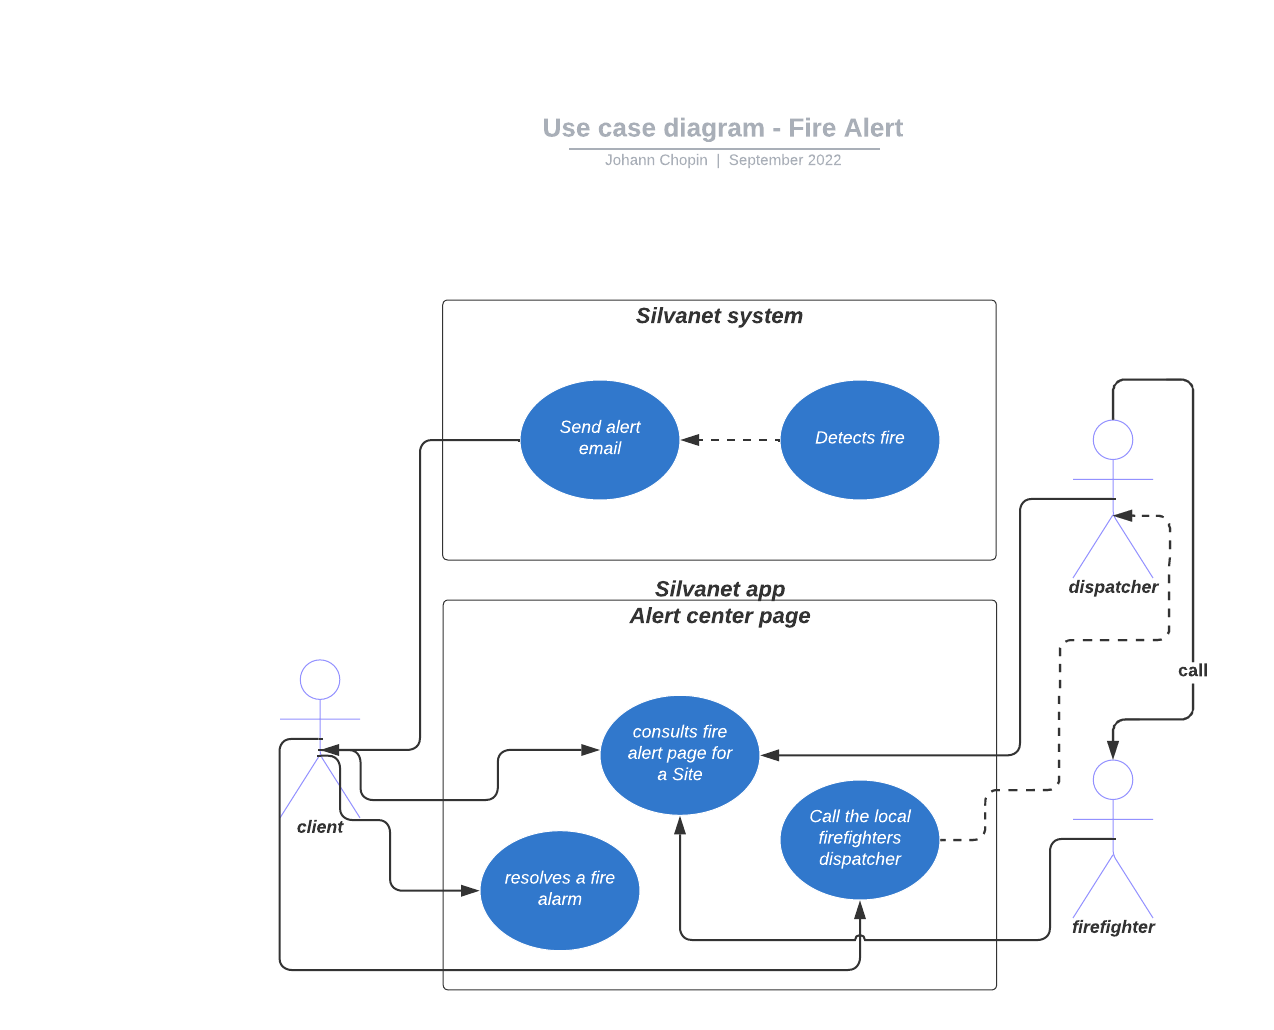
\includegraphics[width=\textwidth]{use_case_diagram_dispatcher}
  \caption{Use-case-diagram, das Kunden, Dispatchers, Feuerwehrleute, das Silvanet-System (Netzwerk von Sensoren im Wald) und die Silvanet-Anwendung bei der Erkennung eines Waldbrandes verbindet.}
  \label{fig:use_case_diagram_dispatcher}
\end{figure}

Mit dieser Darstellung kann man sehen, dass, auch wenn die Anwendung nicht direkt von Feuerwehrleuten genutzt wird (obwohl es für sie möglich ist, sie zu konsultieren), es notwendig ist, dass die Schnittstelle dem Benutzer relevante Informationen anzeigt, sodass er sie kurz und bündig und schnell an die Dispatchers weitergeben kann.
Daher ist es notwendig, genauer zu wissen, was die Feuerwehrleute wissen müssen und wie sie in einer Notsituation wie einem Waldbrand vorgehen.
Da wir keine relevanten Ressourcen gefunden haben, die alle Fragen beantworten, die eine Verbesserung der Silvanet-Schnittstelle ermöglichen, ist eine interne Suche erforderlich.

\subsection{Definition des Fragebogenumfangs}

Wie bei allen Benutzertests ist es notwendig, vorab festzulegen, was das Ziel der Untersuchung ist und wie es erreicht werden soll.
In diesem Sinne war es auch notwendig, dass Entscheidungen von der Gruppe und nicht von Einzelpersonen getroffen wurden, um so viele Ideen wie möglich abzudecken.
Außerdem war noch nicht klar, welches Medium für die Untersuchung verwendet werden sollte, und es gab viele Möglichkeiten, Informationen zu sammeln, z. B. Interviews, Fragebögen oder A/B-Vergleichstests.
Ein von \citeauthor{customerQuestionBoard} entwickeltes Framework für UX-Forschung namens \citetitle{customerQuestionBoard} ermöglicht es, das Problem mit Hilfe von Brainstorming-Sitzungen im Team zu entwirren und ein geeignetes Medium für die Forschung zu definieren.
Diese Methode ist in 7 Schritte unterteilt:

\begin{enumerate}
  \item \textbf{Vorbereitung}: Der erste Schritt besteht darin, sicherzustellen, dass das Team das Ziel der Forschung versteht und weiß, welche Art von Rückmeldungen sie liefern soll.
  \item \textbf{Eingabeaufforderung}: Bitten Sie das Team, Fragen auf Klebezettel zu schreiben, einen Klebezettel pro Frage. Die Frage sollte auf die Frage "Was wollen wir über Feuerwehrleute lernen?
  \item \textbf{Diskutieren und Clustern}: Bitten Sie jeden Benutzer einzeln, seine Klebezettel nach passenden Kategorien zu gruppieren. Die Idee ist zu sehen, wie Fragen auf viele verschiedene Arten gestellt werden können.
  \item \textbf{Einstellung und Verhalten}: Fragen Sie das Team für jedes Cluster, ob sich die Frage auf die Einstellung oder das Verhalten des Kunden bezieht who \textit{Einstellung} ist das, was Menschen über ein Produkt oder eine Dienstleistung sagen oder denken und \textit{Verhalten} ist das, was Menschen mit dem Produkt oder tun ist. Stellen Sie Einstellungsfragen auf der linken Seite und Verhaltensfragen auf der rechten Seite.
  \item \textbf{Qualitativ und quantitativ}: Fragen Sie das Team, ob es bei den Fragenbündeln darum geht, herauszufinden, warum etwas passiert und wie man es beheben kann (qualitative Fragen). Oder darum, wie oft oder wie viel etwas passiert (quantitative Fragen). Danach stellen Sie quantitative Fragen auf der rechten Seite und qualitative Fragen auf der linken Seite.
  \item \textbf{Priorität festlegen}: Im vorherigen Punkt wurden die Fragecluster in vier Gruppen eingeteilt. Das Team muss nun festlegen, welche Gruppe am relevantesten ist.
  \item \textbf{Fragen zu Methoden und Hilfsmitteln zuordnen}: Für das Cluster, das die meisten Stimmen erhalten hat, kann das Team nun herausfinden, welche Nutzerforschungsmethode es anwenden soll. Das Cluster oben rechts verwendet qualitative und strukturierte Methoden. Das Cluster oben links verwendet qualitative und unstrukturierte Methoden. Der untere linke Quadrant verwendet qualitative und indirekte Methoden. Der untere rechte Quadrant verwendet quantitative und indirekte Methoden.
\end{enumerate}

Die Aktivierung wurde vom Dryad Cloud-Team mit dem Miro-Tool durchgeführt. Das Ergebnis ist das folgende Clustering. Die einzelnen Schritte des Prozesses können im Anhang \ref{appendix:question_board} nachgelesen werden.

\begin{figure}[H]
  \centering
  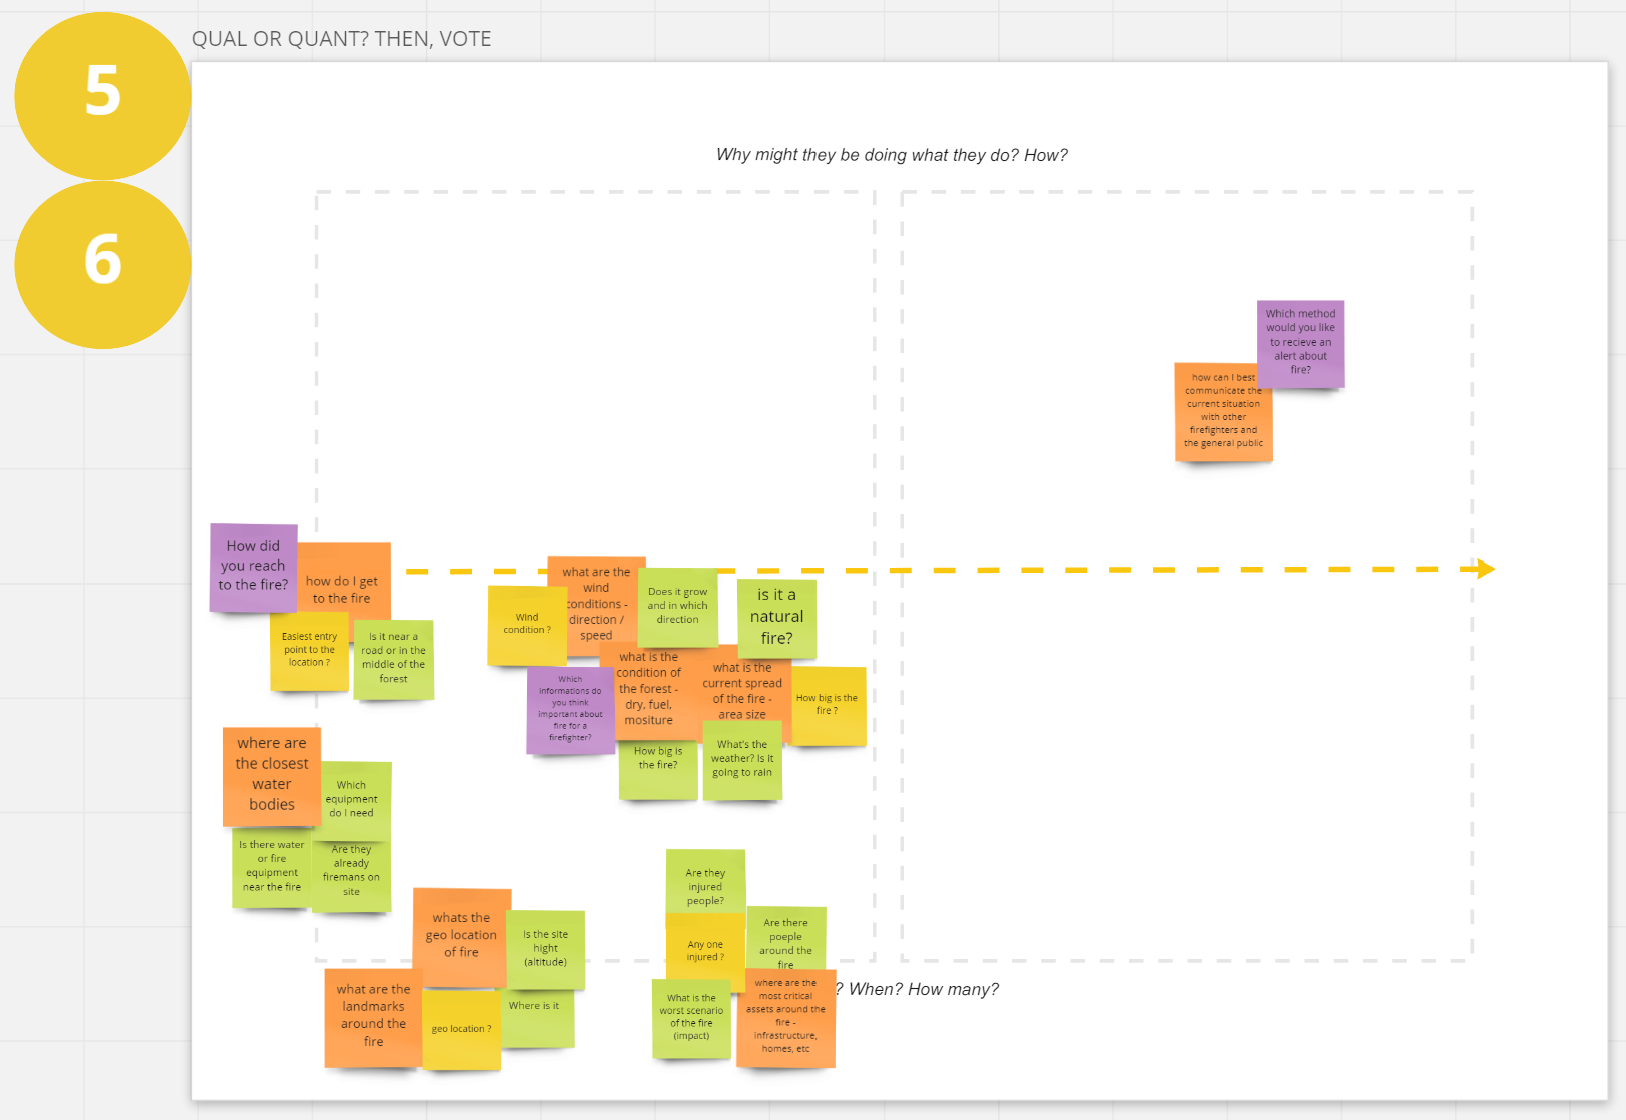
\includegraphics[width=\textwidth]{question_board_5}
  \caption{Ergebnis der UX-Methode des Question Board}
  \label{fig:question_board_5_not_appendix}
\end{figure}

Da sich das Ziel des Boards auf Fragen konzentriert, die sich Feuerwehrleute stellen, ist es nicht verwunderlich, dass sich die meisten Cluster im linken und unteren Teil des Boards konzentrieren.
Das Framework sagt, dass wir uns damit im Bereich der Entdeckung und Befragung des Nutzers befinden.
Dies zeigt uns auch, dass ein strukturierter, indirekter und schriftlicher Fragebogen eine sinnvolle Methode wäre, um diese Fragen zu beantworten\cite{customerQuestionBoard}.

Nachdem die Unterstützung etabliert ist, bleibt die Frage, was man einen Feuerwehrmann fragen kann, um die Waldbrandwarnseite in der Silvanet-Anwendung zu verbessern.
Die verschiedenen Cluster, die durch die verschiedenen Fragen gebildet wurden, die von jedem Mitglied während der Aktivität gestellt wurden, heben die folgenden Interogationen hervor:

\begin{enumerate}
  \item Welche Informationen sind bei der Bekämpfung von Waldbränden hilfreich?
  \item Welche Art von Informationen sind hilfreich, um einen Waldbrand zu erreichen?
  \item Welche Informationen sind für die Vorbereitung eines Einsatzes bei Waldbränden hilfreich?
  \item Wie teilen Sie die Entwicklung des Feuers mit den Behörden/Zivilisten?
  \item Wie teilen Sie die Information mit, dass das Feuer vollständig gelöscht ist?
  \item Welche Art von Informationen sind hilfreich, um den Verlauf des Brandes zu verstehen?
  \item Welche Art von Informationen sind für die Zivilbevölkerung nach dem Erlöschen des Feuers hilfreich?
\end{enumerate}

Das Ziel des Fragebogens ist es daher, möglichst viele Antworten von verschiedenen Personen auf diese Fragen zu erhalten.

\subsection{Aufbau des Fragebogens}

Die Fragen, die so gestellt werden, wie sie sind, sind sehr offen und sie so zu stellen, wie sie sind, mit einem Eingabefeld, würde es wahrscheinlich ermöglichen, qualitativ hochwertige Antworten zu erhalten, die es erlauben, auf andere Fragen zu antworten, die bei der Gestaltung des Formulars nicht einmal angedacht waren.
Es ist jedoch erwiesen, dass die Aufforderung an den Nutzer, qualitative Antworten manuell einzutippen, die Antwortquote des Fragebogens drastisch senkt, je nachdem, wie viele Fragen gestellt werden\cite{userSurveys}.
Da Dryad nicht über die Mittel verfügt, jedem Teilnehmer eine Belohnung zukommen zu lassen, werden die Antworten auf freiwilliger Basis von der Feuerwehrgemeinschaft gegeben.
Mit dieser Bedingung muss der Fragebogen bestimmte Voraussetzungen erfüllen, um attraktiv zu sein und eine gute Rücklaufquote zu bieten.

So ist es relevant, Fragen mit eingeschränkten Antworten zu stellen wodurch das Ausfüllen des Formulars durch den Nutzer schneller geht, die Analyse einfacher wird und die Daten quantifiziert werden können.
Das Ausfüllen des Formulars sollte nicht länger als 7-8 Minuten dauern, da die Abbruchrate bei jeder neuen Frage danach massiv ansteigt\cite{surveyMonkey}.
Eine Technik, die dazu beiträgt, dass der Benutzer bis zum Ende des Formulars antwortet, ist der so genannte \textit{Trichter}, bei dem Sie zu Beginn grundlegende, allgemeine Fragen stellen, in der Mitte komplexere Fragen und am Ende wieder zu allgemeinen Fragen zurückkehren.

Ein weiterer wichtiger Punkt, der bei der Erstellung dieses Formulars zu beachten ist, ist die Sicherheit vor Bias.
Da die Antwortmöglichkeiten begrenzt sind, muss sichergestellt werden, dass alle möglichen Antwortmöglichkeiten abgedeckt sind.
Da dies natürlich nicht möglich ist, muss jede Frage ein optionales Eingabefeld enthalten, in dem der Nutzer eine Bewertung abgeben kann, wenn er der Meinung ist, dass die vorgeschlagenen Antworten nicht die relevantesten sind.

Die Fragen des Formulars werden in vier Themenbereiche unterteilt.

\begin{table}[H]
  \begin{tabular}{p{0.4\linewidth} |p{0.6\linewidth}}
    Thema                                              & Beschreibung                                                                                                                           \\ \hline\hline

    \textbf{Über Sie}                                  & Frage, mit der Sie mehr über das Dienstalter und den Standort des Feuerwehrmanns erfahren können, um das Formular langsam zu beginnen. \\\hline
    \textbf{Herausforderungen bei der Feuerbekämpfung} & Fragen, die sich aus dem Question Board ergeben und von 1 bis 3 reichen.                                                               \\\hline
    \textbf{Verwaltung nach dem Brand}                 & Fragen, die sich aus dem Question Board ergeben und von 4 bis 7 reichen.                                                               \\\hline
    \textbf{Rolle elektronischer Geräte}               & Weniger intensive Fragen zum Einsatz von elektronischen Hilfsmitteln für erfolgreiche Missionen.
  \end{tabular}
  \caption{Unterschiedliche thematische Schwerpunkte des Fragebogens, die eine Trichterstruktur ermöglichen}
\end{table}

Das Formular besteht also aus Textarea für die manuelle Eingabe durch den Benutzer, aus Checkboxen und Radiobuttons für eine eingeschränkte Auswahl mit einer Auswahlmöglichkeit ``andere'' und aus Multiple-Choice-Rastern, die für jede Zeile eine andere Antwort anbieten, und in der Spalte eine Skala von \textbf{1} bis \textbf{7}, um die Relevanz der Antwort zu bewerten, wobei 1 \textbf{unnötig} und 7 \textbf{notwendig} ist.

\begin{figure}[H]
  \centering
  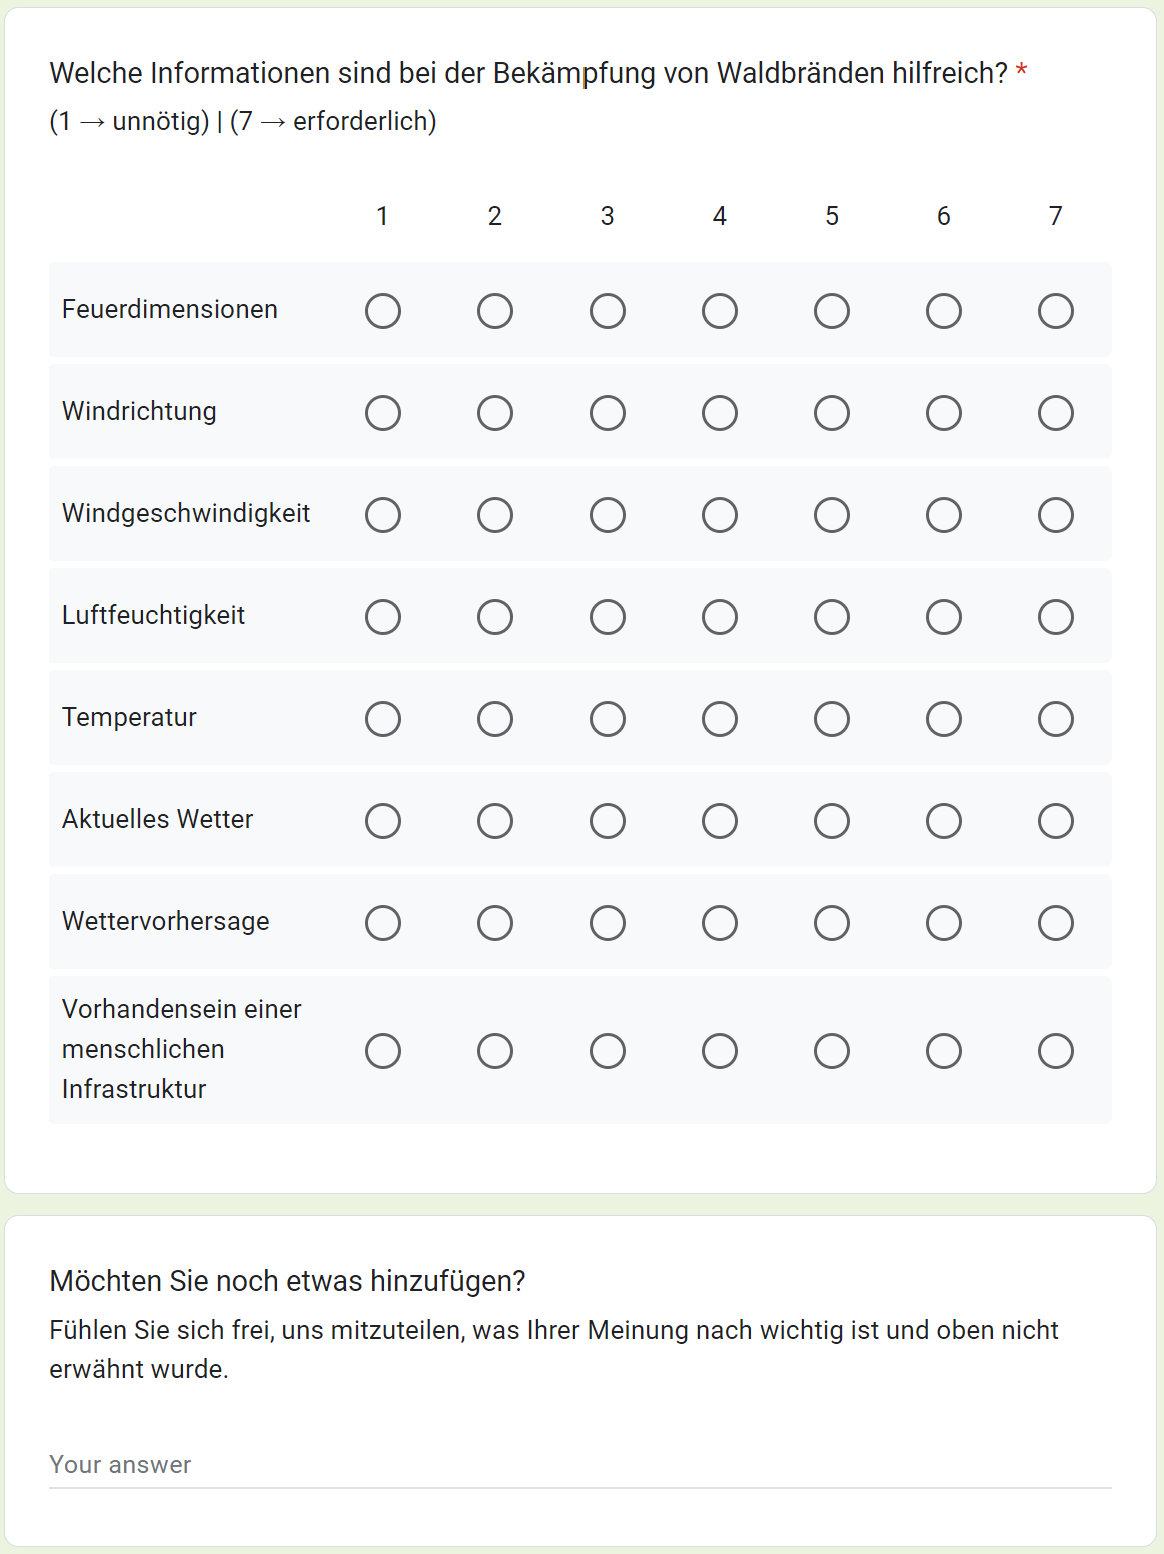
\includegraphics[width=12cm]{survey_response_grid}
  \caption{Beispiel einer Frage mit Multiple-Choice-Rastern mit der Möglichkeit, Details hinzuzufügen aus dem Formular für die Feuerwehr}
  \label{fig:survey_response_grid}
\end{figure}

Das Formular sollte auf der ganzen Welt verbreitet werden, um möglichst viele und möglichst unterschiedliche Antworten zu erhalten.
Daher wurde das Formular in die drei Sprachen Englisch, Deutsch und Französisch übersetzt.
Das deutsche Formular finden Sie im Anhang \ref{appendix:firefighter-survey}.

\subsection{Teilen des Fragebogens}

Nun, da das Formular die relevanten Fragen enthält, nicht verzerrt ist und weniger als sieben Minuten dauert, muss es noch geteilt werden.
Das Zielpublikum sind Gruppen von Feuerwehrleuten, die den Fragebogen dann an Bekannte weitergeben könnten.
Da ich keine Vorkenntnisse in diesem Bereich hatte, musste ich das Formular über das klassische Netzwerk teilen.
Die verwendeten Zielplattformen waren:

\begin{itemize}
  \item die Linkedin-Verbindungen
  \item Feuerwehrgruppen auf Reddit
  \item Feuerwehrgruppen auf Facebook
  \item Kontaktseite verschiedener Feuerwehrforen
  \item gezieltes Versenden von E-Mails an Feuerwehradressen
\end{itemize}

Die erste Annäherung erfolgte über den Namen des Unternehmens direkt, das in der Branche innovativ sein wollte und nach professionellem Feedback suchte.
Dennoch war der Empfang durch die Gemeinde nicht sehr herzlich, sodass wir unsere Strategie ändern mussten.
So musste ich den Fragebogen persönlich weitergeben und auf seine Bedeutung für meine Thesis hinweisen.
Diese Vorgehensweise kam besser an und führte zu guten Antworten.

\subsection{Ergebnis des Fragebogens}

Um im Zeitplan zu bleiben, wurde beschlossen, dass etwa 60 Antworten ausreichen würden, um eine Analyse der ersten Bedürfnisse der Feuerwehr zu erstellen.
Die verarbeiteten Antworten können in Form von Grafiken im Anhang \ref{appendix:firefighter_survey} eingesehen werden.

Die wichtigste Erkenntnis aus dieser Untersuchung für das Produkt von Dryad ist, dass die Schnittstelle in der Lage ist, den Austausch von Informationen vom Kunden an die Feuerwehr zu erleichtern, aber auch von der Schnittstelle direkt an die Feuerwehr.
Die meisten Feuerwehrleute nutzen Tablets und Smartphones \ref{fig:survey_graph_devices_mission}, um Echtzeitinformationen über Karten und Wetter zu erhalten \ref{fig:survey_graph_device_features}.
Darüber hinaus erfolgt der Informationsaustausch zwischen Feuerwehrleuten und Außenstehenden zunehmend digital über soziale Netzwerke und Community-Websites \ref{fig:survey_graph_share_extinction} \ref{fig:survey_graph_share_evolution}.
Ein Verbesserungspunkt der Silvanet-Schnittstelle wäre also, dass man relevante Inhalte des entdeckten Waldbrandes einfach an die Zivilbevölkerung weitergeben könnte, und zwar durch Standards wie ein Übersichtsbild, eine PDF-Datei mit weiterführenden Details oder einen öffentlichen Link zur Seite des Warnzentrums, der es jedem ermöglicht, den Verlauf des Feuers auf der interaktiven Karte in Echtzeit zu verfolgen.
Was zunächst relevant zu sein scheint, sind die Risiken für die Menschen in der Nähe des Feuers, z. B. ob ein Feuer wieder aufflammen kann oder ob Giftstoffe vorhanden sind, sowie die Kartografie des vom Feuer betroffenen Gebiets.

Was die Feuerwehr direkt betrifft, sollte das Interface in der Lage sein, die Windrichtung auf verschiedenen interaktiven Karten anzuzeigen \ref{fig:survey_graph_progression}, eine Wettervorhersage zu machen und anzuzeigen \ref{fig:survey_graph_tackling}, ob sich Häuser oder menschliche Strukturen in der Nähe des Brandherdes befinden oder nicht \ref{fig:survey_graph_tackling}.
In einer zweiten Iteration könnte die Schnittstelle Funktionen zur Anzeige der Größe des Waldbrandes, der Bodenzusammensetzung am Brandort, des Vorhandenseins von Wasserreserven in der Nähe des Brandortes \ref{fig:survey_graph_prepare} und des Vorhandenseins eines Weges oder einer Straße zum Brandort bereitstellen \ref{fig:survey_graph_reach_fire}.

Diese Ergebnisse sind auch insofern von Vorteil, als die Warnseite der Anwendung und die an den Kunden gesendete Warnmail die wichtigsten Informationen auf einfache Weise enthalten und so eine direkte und schnelle Kommunikation mit den Dispatchers ermöglichen.